% Created by tikzDevice version 0.7.0 on 2014-07-29 12:45:02
% !TEX encoding = UTF-8 Unicode
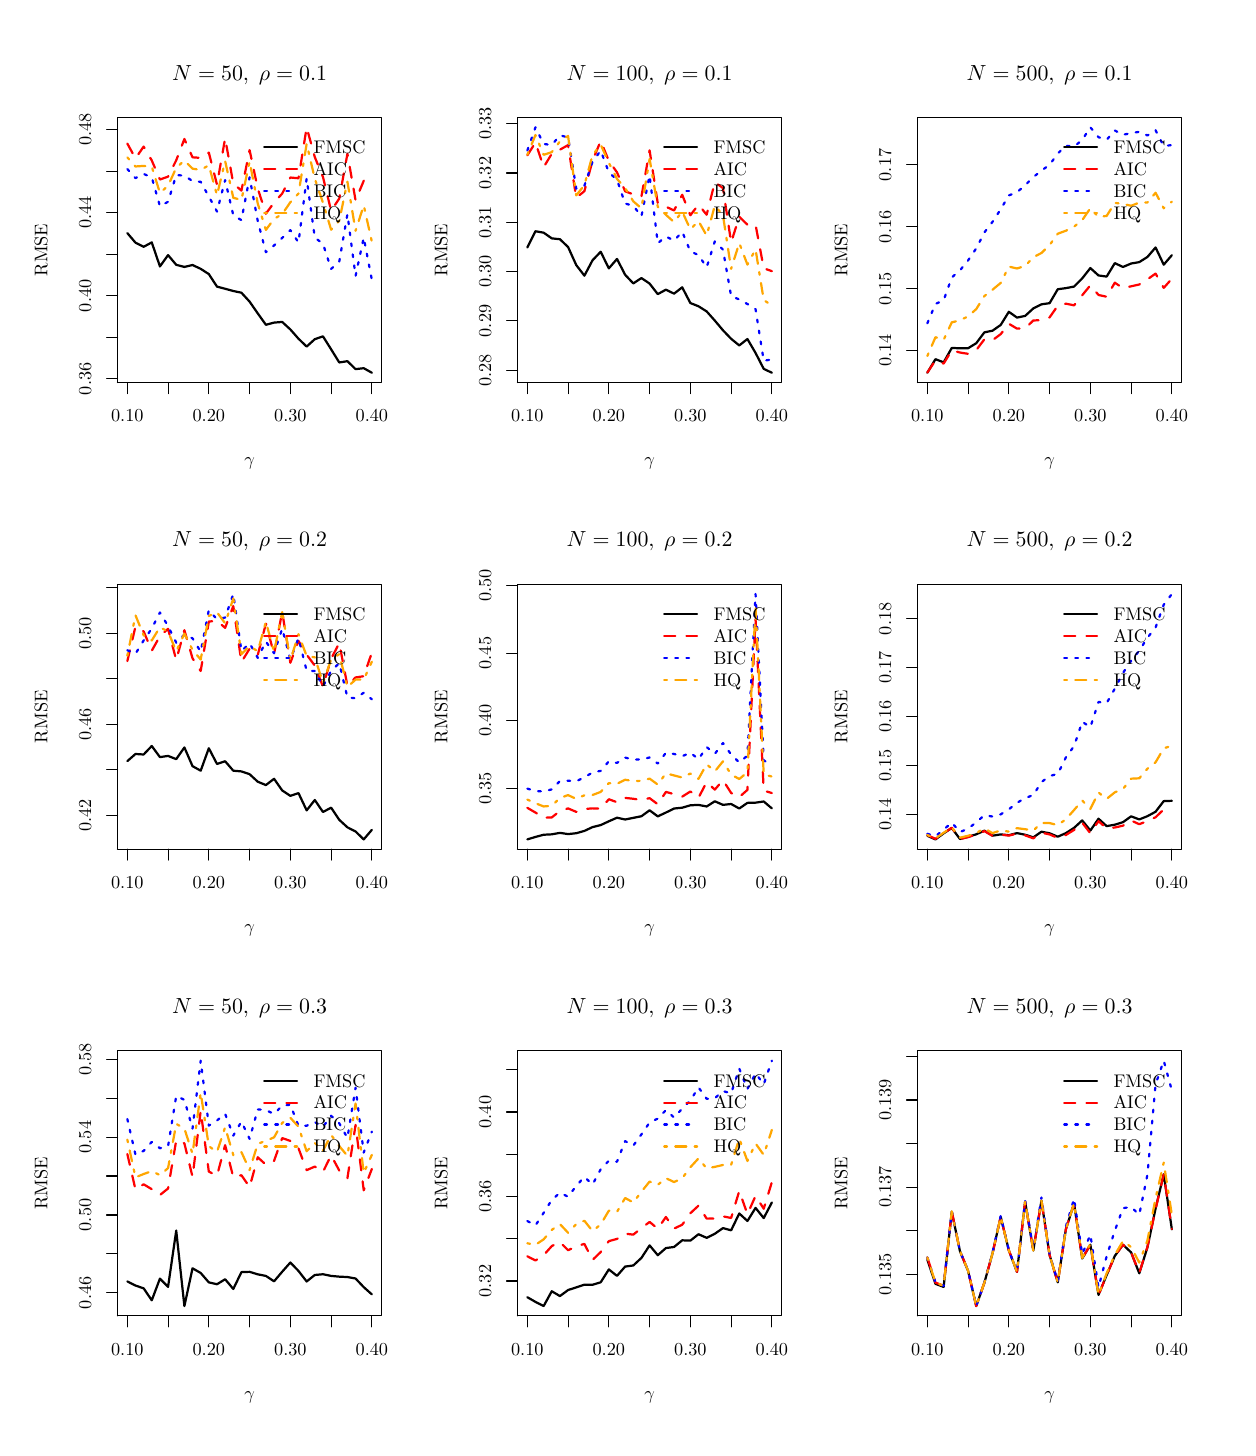
\begin{tikzpicture}[x=1pt,y=1pt]
\definecolor[named]{fillColor}{rgb}{1.00,1.00,1.00}
\path[use as bounding box,fill=fillColor,fill opacity=0.00] (0,0) rectangle (433.62,505.89);
\begin{scope}
\path[clip] ( 32.47,377.65) rectangle (127.91,473.42);
\definecolor[named]{drawColor}{rgb}{0.00,0.00,0.00}

\path[draw=drawColor,line width= 0.8pt,line join=round,line cap=round] ( 36.01,431.66) --
	( 38.95,428.20) --
	( 41.90,426.70) --
	( 44.84,428.29) --
	( 47.79,419.61) --
	( 50.73,423.70) --
	( 53.68,420.19) --
	( 56.63,419.43) --
	( 59.57,420.12) --
	( 62.52,418.74) --
	( 65.46,416.84) --
	( 68.41,412.31) --
	( 71.35,411.54) --
	( 74.30,410.73) --
	( 77.24,410.11) --
	( 80.19,406.89) --
	( 83.14,402.64) --
	( 86.08,398.52) --
	( 89.03,399.31) --
	( 91.97,399.55) --
	( 94.92,396.83) --
	( 97.86,393.49) --
	(100.81,390.65) --
	(103.75,393.32) --
	(106.70,394.35) --
	(109.65,389.66) --
	(112.59,384.91) --
	(115.54,385.37) --
	(118.48,382.50) --
	(121.43,382.83) --
	(124.37,381.20);
\end{scope}
\begin{scope}
\path[clip] (  0.00,  0.00) rectangle (433.62,505.89);
\definecolor[named]{drawColor}{rgb}{0.00,0.00,0.00}

\path[draw=drawColor,line width= 0.4pt,line join=round,line cap=round] ( 36.01,377.65) -- (124.37,377.65);

\path[draw=drawColor,line width= 0.4pt,line join=round,line cap=round] ( 36.01,377.65) -- ( 36.01,373.69);

\path[draw=drawColor,line width= 0.4pt,line join=round,line cap=round] ( 50.73,377.65) -- ( 50.73,373.69);

\path[draw=drawColor,line width= 0.4pt,line join=round,line cap=round] ( 65.46,377.65) -- ( 65.46,373.69);

\path[draw=drawColor,line width= 0.4pt,line join=round,line cap=round] ( 80.19,377.65) -- ( 80.19,373.69);

\path[draw=drawColor,line width= 0.4pt,line join=round,line cap=round] ( 94.92,377.65) -- ( 94.92,373.69);

\path[draw=drawColor,line width= 0.4pt,line join=round,line cap=round] (109.65,377.65) -- (109.65,373.69);

\path[draw=drawColor,line width= 0.4pt,line join=round,line cap=round] (124.37,377.65) -- (124.37,373.69);

\node[text=drawColor,anchor=base,inner sep=0pt, outer sep=0pt, scale=  0.66] at ( 36.01,363.40) {0.10};

\node[text=drawColor,anchor=base,inner sep=0pt, outer sep=0pt, scale=  0.66] at ( 65.46,363.40) {0.20};

\node[text=drawColor,anchor=base,inner sep=0pt, outer sep=0pt, scale=  0.66] at ( 94.92,363.40) {0.30};

\node[text=drawColor,anchor=base,inner sep=0pt, outer sep=0pt, scale=  0.66] at (124.37,363.40) {0.40};

\path[draw=drawColor,line width= 0.4pt,line join=round,line cap=round] ( 32.47,378.98) -- ( 32.47,469.05);

\path[draw=drawColor,line width= 0.4pt,line join=round,line cap=round] ( 32.47,378.98) -- ( 28.51,378.98);

\path[draw=drawColor,line width= 0.4pt,line join=round,line cap=round] ( 32.47,393.99) -- ( 28.51,393.99);

\path[draw=drawColor,line width= 0.4pt,line join=round,line cap=round] ( 32.47,409.01) -- ( 28.51,409.01);

\path[draw=drawColor,line width= 0.4pt,line join=round,line cap=round] ( 32.47,424.02) -- ( 28.51,424.02);

\path[draw=drawColor,line width= 0.4pt,line join=round,line cap=round] ( 32.47,439.03) -- ( 28.51,439.03);

\path[draw=drawColor,line width= 0.4pt,line join=round,line cap=round] ( 32.47,454.04) -- ( 28.51,454.04);

\path[draw=drawColor,line width= 0.4pt,line join=round,line cap=round] ( 32.47,469.05) -- ( 28.51,469.05);

\node[text=drawColor,rotate= 90.00,anchor=base,inner sep=0pt, outer sep=0pt, scale=  0.66] at ( 22.97,378.98) {0.36};

\node[text=drawColor,rotate= 90.00,anchor=base,inner sep=0pt, outer sep=0pt, scale=  0.66] at ( 22.97,409.01) {0.40};

\node[text=drawColor,rotate= 90.00,anchor=base,inner sep=0pt, outer sep=0pt, scale=  0.66] at ( 22.97,439.03) {0.44};

\node[text=drawColor,rotate= 90.00,anchor=base,inner sep=0pt, outer sep=0pt, scale=  0.66] at ( 22.97,469.05) {0.48};

\path[draw=drawColor,line width= 0.4pt,line join=round,line cap=round] ( 32.47,377.65) --
	(127.91,377.65) --
	(127.91,473.42) --
	( 32.47,473.42) --
	( 32.47,377.65);
\end{scope}
\begin{scope}
\path[clip] (  0.00,337.26) rectangle (144.54,505.89);
\definecolor[named]{drawColor}{rgb}{0.00,0.00,0.00}

\node[text=drawColor,anchor=base,inner sep=0pt, outer sep=0pt, scale=  0.79] at ( 80.19,486.92) {\bfseries $N=50, \;\rho=0.1$};

\node[text=drawColor,anchor=base,inner sep=0pt, outer sep=0pt, scale=  0.66] at ( 80.19,347.56) {$\gamma$};

\node[text=drawColor,rotate= 90.00,anchor=base,inner sep=0pt, outer sep=0pt, scale=  0.66] at (  7.13,425.53) {RMSE};
\end{scope}
\begin{scope}
\path[clip] ( 32.47,377.65) rectangle (127.91,473.42);
\definecolor[named]{drawColor}{rgb}{1.00,0.00,0.00}

\path[draw=drawColor,line width= 0.8pt,dash pattern=on 4pt off 4pt ,line join=round,line cap=round] ( 36.01,464.01) --
	( 38.95,458.63) --
	( 41.90,462.91) --
	( 44.84,457.91) --
	( 47.79,451.02) --
	( 50.73,452.06) --
	( 53.68,457.97) --
	( 56.63,465.66) --
	( 59.57,459.04) --
	( 62.52,458.83) --
	( 65.46,460.74) --
	( 68.41,449.16) --
	( 71.35,465.93) --
	( 74.30,449.56) --
	( 77.24,447.01) --
	( 80.19,461.65) --
	( 83.14,447.74) --
	( 86.08,438.67) --
	( 89.03,442.68) --
	( 91.97,445.93) --
	( 94.92,451.74) --
	( 97.86,451.47) --
	(100.81,469.87) --
	(103.75,459.13) --
	(106.70,451.95) --
	(109.65,439.71) --
	(112.59,444.13) --
	(115.54,460.33) --
	(118.48,443.51) --
	(121.43,450.53) --
	(124.37,453.15);
\definecolor[named]{drawColor}{rgb}{0.00,0.00,1.00}

\path[draw=drawColor,line width= 0.8pt,dash pattern=on 1pt off 3pt ,line join=round,line cap=round] ( 36.01,454.80) --
	( 38.95,451.52) --
	( 41.90,453.04) --
	( 44.84,451.78) --
	( 47.79,441.36) --
	( 50.73,442.97) --
	( 53.68,452.64) --
	( 56.63,452.40) --
	( 59.57,450.47) --
	( 62.52,450.19) --
	( 65.46,444.87) --
	( 68.41,439.45) --
	( 71.35,450.81) --
	( 74.30,438.11) --
	( 77.24,436.34) --
	( 80.19,451.82) --
	( 83.14,435.99) --
	( 86.08,424.74) --
	( 89.03,427.19) --
	( 91.97,429.93) --
	( 94.92,432.72) --
	( 97.86,428.25) --
	(100.81,451.41) --
	(103.75,430.01) --
	(106.70,427.81) --
	(109.65,418.72) --
	(112.59,421.35) --
	(115.54,438.47) --
	(118.48,416.15) --
	(121.43,430.04) --
	(124.37,414.77);
\definecolor[named]{drawColor}{rgb}{1.00,0.65,0.00}

\path[draw=drawColor,line width= 0.8pt,dash pattern=on 1pt off 3pt on 4pt off 3pt ,line join=round,line cap=round] ( 36.01,459.02) --
	( 38.95,455.73) --
	( 41.90,455.93) --
	( 44.84,455.68) --
	( 47.79,446.14) --
	( 50.73,448.77) --
	( 53.68,455.26) --
	( 56.63,457.88) --
	( 59.57,454.94) --
	( 62.52,454.48) --
	( 65.46,456.16) --
	( 68.41,445.33) --
	( 71.35,457.70) --
	( 74.30,444.41) --
	( 77.24,443.64) --
	( 80.19,457.52) --
	( 83.14,442.35) --
	( 86.08,432.81) --
	( 89.03,436.80) --
	( 91.97,438.48) --
	( 94.92,442.82) --
	( 97.86,445.96) --
	(100.81,463.93) --
	(103.75,451.32) --
	(106.70,442.63) --
	(109.65,432.87) --
	(112.59,436.12) --
	(115.54,450.24) --
	(118.48,432.48) --
	(121.43,441.67) --
	(124.37,428.57);
\definecolor[named]{drawColor}{rgb}{0.00,0.00,0.00}

\path[draw=drawColor,line width= 0.8pt,line join=round,line cap=round] ( 85.47,462.63) -- ( 97.35,462.63);
\definecolor[named]{drawColor}{rgb}{1.00,0.00,0.00}

\path[draw=drawColor,line width= 0.8pt,dash pattern=on 4pt off 4pt ,line join=round,line cap=round] ( 85.47,454.71) -- ( 97.35,454.71);
\definecolor[named]{drawColor}{rgb}{0.00,0.00,1.00}

\path[draw=drawColor,line width= 0.8pt,dash pattern=on 1pt off 3pt ,line join=round,line cap=round] ( 85.47,446.79) -- ( 97.35,446.79);
\definecolor[named]{drawColor}{rgb}{1.00,0.65,0.00}

\path[draw=drawColor,line width= 0.8pt,dash pattern=on 1pt off 3pt on 4pt off 3pt ,line join=round,line cap=round] ( 85.47,438.87) -- ( 97.35,438.87);
\definecolor[named]{drawColor}{rgb}{0.00,0.00,0.00}

\node[text=drawColor,anchor=base west,inner sep=0pt, outer sep=0pt, scale=  0.66] at (103.29,460.35) {FMSC};

\node[text=drawColor,anchor=base west,inner sep=0pt, outer sep=0pt, scale=  0.66] at (103.29,452.43) {AIC};

\node[text=drawColor,anchor=base west,inner sep=0pt, outer sep=0pt, scale=  0.66] at (103.29,444.51) {BIC};

\node[text=drawColor,anchor=base west,inner sep=0pt, outer sep=0pt, scale=  0.66] at (103.29,436.59) {HQ};
\end{scope}
\begin{scope}
\path[clip] (177.01,377.65) rectangle (272.45,473.42);
\definecolor[named]{drawColor}{rgb}{0.00,0.00,0.00}

\path[draw=drawColor,line width= 0.8pt,line join=round,line cap=round] (180.55,426.45) --
	(183.49,432.32) --
	(186.44,431.81) --
	(189.38,429.75) --
	(192.33,429.44) --
	(195.27,426.63) --
	(198.22,420.11) --
	(201.17,416.27) --
	(204.11,421.83) --
	(207.06,424.91) --
	(210.00,418.91) --
	(212.95,422.31) --
	(215.89,416.59) --
	(218.84,413.47) --
	(221.78,415.41) --
	(224.73,413.41) --
	(227.68,409.60) --
	(230.62,411.20) --
	(233.57,409.78) --
	(236.51,412.06) --
	(239.46,406.38) --
	(242.40,405.21) --
	(245.35,403.35) --
	(248.29,400.05) --
	(251.24,396.54) --
	(254.19,393.46) --
	(257.13,391.07) --
	(260.08,393.38) --
	(263.02,388.34) --
	(265.97,382.59) --
	(268.91,381.20);
\end{scope}
\begin{scope}
\path[clip] (  0.00,  0.00) rectangle (433.62,505.89);
\definecolor[named]{drawColor}{rgb}{0.00,0.00,0.00}

\path[draw=drawColor,line width= 0.4pt,line join=round,line cap=round] (180.55,377.65) -- (268.91,377.65);

\path[draw=drawColor,line width= 0.4pt,line join=round,line cap=round] (180.55,377.65) -- (180.55,373.69);

\path[draw=drawColor,line width= 0.4pt,line join=round,line cap=round] (195.27,377.65) -- (195.27,373.69);

\path[draw=drawColor,line width= 0.4pt,line join=round,line cap=round] (210.00,377.65) -- (210.00,373.69);

\path[draw=drawColor,line width= 0.4pt,line join=round,line cap=round] (224.73,377.65) -- (224.73,373.69);

\path[draw=drawColor,line width= 0.4pt,line join=round,line cap=round] (239.46,377.65) -- (239.46,373.69);

\path[draw=drawColor,line width= 0.4pt,line join=round,line cap=round] (254.19,377.65) -- (254.19,373.69);

\path[draw=drawColor,line width= 0.4pt,line join=round,line cap=round] (268.91,377.65) -- (268.91,373.69);

\node[text=drawColor,anchor=base,inner sep=0pt, outer sep=0pt, scale=  0.66] at (180.55,363.40) {0.10};

\node[text=drawColor,anchor=base,inner sep=0pt, outer sep=0pt, scale=  0.66] at (210.00,363.40) {0.20};

\node[text=drawColor,anchor=base,inner sep=0pt, outer sep=0pt, scale=  0.66] at (239.46,363.40) {0.30};

\node[text=drawColor,anchor=base,inner sep=0pt, outer sep=0pt, scale=  0.66] at (268.91,363.40) {0.40};

\path[draw=drawColor,line width= 0.4pt,line join=round,line cap=round] (177.01,382.11) -- (177.01,471.20);

\path[draw=drawColor,line width= 0.4pt,line join=round,line cap=round] (177.01,382.11) -- (173.05,382.11);

\path[draw=drawColor,line width= 0.4pt,line join=round,line cap=round] (177.01,399.93) -- (173.05,399.93);

\path[draw=drawColor,line width= 0.4pt,line join=round,line cap=round] (177.01,417.75) -- (173.05,417.75);

\path[draw=drawColor,line width= 0.4pt,line join=round,line cap=round] (177.01,435.57) -- (173.05,435.57);

\path[draw=drawColor,line width= 0.4pt,line join=round,line cap=round] (177.01,453.38) -- (173.05,453.38);

\path[draw=drawColor,line width= 0.4pt,line join=round,line cap=round] (177.01,471.20) -- (173.05,471.20);

\node[text=drawColor,rotate= 90.00,anchor=base,inner sep=0pt, outer sep=0pt, scale=  0.66] at (167.51,382.11) {0.28};

\node[text=drawColor,rotate= 90.00,anchor=base,inner sep=0pt, outer sep=0pt, scale=  0.66] at (167.51,399.93) {0.29};

\node[text=drawColor,rotate= 90.00,anchor=base,inner sep=0pt, outer sep=0pt, scale=  0.66] at (167.51,417.75) {0.30};

\node[text=drawColor,rotate= 90.00,anchor=base,inner sep=0pt, outer sep=0pt, scale=  0.66] at (167.51,435.57) {0.31};

\node[text=drawColor,rotate= 90.00,anchor=base,inner sep=0pt, outer sep=0pt, scale=  0.66] at (167.51,453.38) {0.32};

\node[text=drawColor,rotate= 90.00,anchor=base,inner sep=0pt, outer sep=0pt, scale=  0.66] at (167.51,471.20) {0.33};

\path[draw=drawColor,line width= 0.4pt,line join=round,line cap=round] (177.01,377.65) --
	(272.45,377.65) --
	(272.45,473.42) --
	(177.01,473.42) --
	(177.01,377.65);
\end{scope}
\begin{scope}
\path[clip] (144.54,337.26) rectangle (289.08,505.89);
\definecolor[named]{drawColor}{rgb}{0.00,0.00,0.00}

\node[text=drawColor,anchor=base,inner sep=0pt, outer sep=0pt, scale=  0.79] at (224.73,486.92) {\bfseries $N=100, \;\rho=0.1$};

\node[text=drawColor,anchor=base,inner sep=0pt, outer sep=0pt, scale=  0.66] at (224.73,347.56) {$\gamma$};

\node[text=drawColor,rotate= 90.00,anchor=base,inner sep=0pt, outer sep=0pt, scale=  0.66] at (151.67,425.53) {RMSE};
\end{scope}
\begin{scope}
\path[clip] (177.01,377.65) rectangle (272.45,473.42);
\definecolor[named]{drawColor}{rgb}{1.00,0.00,0.00}

\path[draw=drawColor,line width= 0.8pt,dash pattern=on 4pt off 4pt ,line join=round,line cap=round] (180.55,459.76) --
	(183.49,464.38) --
	(186.44,455.46) --
	(189.38,460.33) --
	(192.33,461.80) --
	(195.27,463.45) --
	(198.22,444.42) --
	(201.17,446.81) --
	(204.11,457.83) --
	(207.06,464.93) --
	(210.00,457.74) --
	(212.95,453.61) --
	(215.89,446.76) --
	(218.84,445.65) --
	(221.78,444.89) --
	(224.73,461.56) --
	(227.68,442.43) --
	(230.62,441.20) --
	(233.57,439.83) --
	(236.51,445.50) --
	(239.46,438.10) --
	(242.40,441.94) --
	(245.35,438.29) --
	(248.29,450.06) --
	(251.24,447.93) --
	(254.19,428.26) --
	(257.13,437.59) --
	(260.08,434.68) --
	(263.02,434.66) --
	(265.97,418.95) --
	(268.91,417.90);
\definecolor[named]{drawColor}{rgb}{0.00,0.00,1.00}

\path[draw=drawColor,line width= 0.8pt,dash pattern=on 1pt off 3pt ,line join=round,line cap=round] (180.55,461.51) --
	(183.49,469.87) --
	(186.44,463.87) --
	(189.38,463.48) --
	(192.33,466.99) --
	(195.27,466.25) --
	(198.22,447.73) --
	(201.17,448.80) --
	(204.11,457.42) --
	(207.06,461.46) --
	(210.00,453.62) --
	(212.95,450.90) --
	(215.89,442.34) --
	(218.84,441.53) --
	(221.78,437.69) --
	(224.73,452.52) --
	(227.68,427.98) --
	(230.62,430.45) --
	(233.57,428.90) --
	(236.51,432.16) --
	(239.46,425.07) --
	(242.40,423.69) --
	(245.35,419.29) --
	(248.29,428.63) --
	(251.24,425.70) --
	(254.19,408.85) --
	(257.13,407.69) --
	(260.08,406.02) --
	(263.02,404.14) --
	(265.97,385.51) --
	(268.91,386.02);
\definecolor[named]{drawColor}{rgb}{1.00,0.65,0.00}

\path[draw=drawColor,line width= 0.8pt,dash pattern=on 1pt off 3pt on 4pt off 3pt ,line join=round,line cap=round] (180.55,460.00) --
	(183.49,467.09) --
	(186.44,459.95) --
	(189.38,460.92) --
	(192.33,464.79) --
	(195.27,466.76) --
	(198.22,445.27) --
	(201.17,449.00) --
	(204.11,459.85) --
	(207.06,463.63) --
	(210.00,457.05) --
	(212.95,451.24) --
	(215.89,447.93) --
	(218.84,443.14) --
	(221.78,440.58) --
	(224.73,458.46) --
	(227.68,441.19) --
	(230.62,438.26) --
	(233.57,435.62) --
	(236.51,439.45) --
	(239.46,432.99) --
	(242.40,436.01) --
	(245.35,430.75) --
	(248.29,441.57) --
	(251.24,438.09) --
	(254.19,418.74) --
	(257.13,428.05) --
	(260.08,420.26) --
	(263.02,425.78) --
	(265.97,407.44) --
	(268.91,405.55);
\definecolor[named]{drawColor}{rgb}{0.00,0.00,0.00}

\path[draw=drawColor,line width= 0.8pt,line join=round,line cap=round] (230.01,462.63) -- (241.89,462.63);
\definecolor[named]{drawColor}{rgb}{1.00,0.00,0.00}

\path[draw=drawColor,line width= 0.8pt,dash pattern=on 4pt off 4pt ,line join=round,line cap=round] (230.01,454.71) -- (241.89,454.71);
\definecolor[named]{drawColor}{rgb}{0.00,0.00,1.00}

\path[draw=drawColor,line width= 0.8pt,dash pattern=on 1pt off 3pt ,line join=round,line cap=round] (230.01,446.79) -- (241.89,446.79);
\definecolor[named]{drawColor}{rgb}{1.00,0.65,0.00}

\path[draw=drawColor,line width= 0.8pt,dash pattern=on 1pt off 3pt on 4pt off 3pt ,line join=round,line cap=round] (230.01,438.87) -- (241.89,438.87);
\definecolor[named]{drawColor}{rgb}{0.00,0.00,0.00}

\node[text=drawColor,anchor=base west,inner sep=0pt, outer sep=0pt, scale=  0.66] at (247.83,460.35) {FMSC};

\node[text=drawColor,anchor=base west,inner sep=0pt, outer sep=0pt, scale=  0.66] at (247.83,452.43) {AIC};

\node[text=drawColor,anchor=base west,inner sep=0pt, outer sep=0pt, scale=  0.66] at (247.83,444.51) {BIC};

\node[text=drawColor,anchor=base west,inner sep=0pt, outer sep=0pt, scale=  0.66] at (247.83,436.59) {HQ};
\end{scope}
\begin{scope}
\path[clip] (321.55,377.65) rectangle (416.99,473.42);
\definecolor[named]{drawColor}{rgb}{0.00,0.00,0.00}

\path[draw=drawColor,line width= 0.8pt,line join=round,line cap=round] (325.09,381.20) --
	(328.03,386.10) --
	(330.98,384.94) --
	(333.92,390.16) --
	(336.87,390.02) --
	(339.81,390.05) --
	(342.76,391.86) --
	(345.71,395.79) --
	(348.65,396.39) --
	(351.60,398.47) --
	(354.54,403.22) --
	(357.49,401.12) --
	(360.43,401.73) --
	(363.38,404.43) --
	(366.32,405.91) --
	(369.27,406.34) --
	(372.22,411.37) --
	(375.16,411.77) --
	(378.11,412.33) --
	(381.05,415.29) --
	(384.00,419.02) --
	(386.94,416.35) --
	(389.89,415.94) --
	(392.83,420.80) --
	(395.78,419.41) --
	(398.73,420.66) --
	(401.67,421.17) --
	(404.62,423.03) --
	(407.56,426.46) --
	(410.51,420.25) --
	(413.45,423.67);
\end{scope}
\begin{scope}
\path[clip] (  0.00,  0.00) rectangle (433.62,505.89);
\definecolor[named]{drawColor}{rgb}{0.00,0.00,0.00}

\path[draw=drawColor,line width= 0.4pt,line join=round,line cap=round] (325.09,377.65) -- (413.45,377.65);

\path[draw=drawColor,line width= 0.4pt,line join=round,line cap=round] (325.09,377.65) -- (325.09,373.69);

\path[draw=drawColor,line width= 0.4pt,line join=round,line cap=round] (339.81,377.65) -- (339.81,373.69);

\path[draw=drawColor,line width= 0.4pt,line join=round,line cap=round] (354.54,377.65) -- (354.54,373.69);

\path[draw=drawColor,line width= 0.4pt,line join=round,line cap=round] (369.27,377.65) -- (369.27,373.69);

\path[draw=drawColor,line width= 0.4pt,line join=round,line cap=round] (384.00,377.65) -- (384.00,373.69);

\path[draw=drawColor,line width= 0.4pt,line join=round,line cap=round] (398.73,377.65) -- (398.73,373.69);

\path[draw=drawColor,line width= 0.4pt,line join=round,line cap=round] (413.45,377.65) -- (413.45,373.69);

\node[text=drawColor,anchor=base,inner sep=0pt, outer sep=0pt, scale=  0.66] at (325.09,363.40) {0.10};

\node[text=drawColor,anchor=base,inner sep=0pt, outer sep=0pt, scale=  0.66] at (354.54,363.40) {0.20};

\node[text=drawColor,anchor=base,inner sep=0pt, outer sep=0pt, scale=  0.66] at (384.00,363.40) {0.30};

\node[text=drawColor,anchor=base,inner sep=0pt, outer sep=0pt, scale=  0.66] at (413.45,363.40) {0.40};

\path[draw=drawColor,line width= 0.4pt,line join=round,line cap=round] (321.55,389.16) -- (321.55,456.29);

\path[draw=drawColor,line width= 0.4pt,line join=round,line cap=round] (321.55,389.16) -- (317.59,389.16);

\path[draw=drawColor,line width= 0.4pt,line join=round,line cap=round] (321.55,411.54) -- (317.59,411.54);

\path[draw=drawColor,line width= 0.4pt,line join=round,line cap=round] (321.55,433.91) -- (317.59,433.91);

\path[draw=drawColor,line width= 0.4pt,line join=round,line cap=round] (321.55,456.29) -- (317.59,456.29);

\node[text=drawColor,rotate= 90.00,anchor=base,inner sep=0pt, outer sep=0pt, scale=  0.66] at (312.05,389.16) {0.14};

\node[text=drawColor,rotate= 90.00,anchor=base,inner sep=0pt, outer sep=0pt, scale=  0.66] at (312.05,411.54) {0.15};

\node[text=drawColor,rotate= 90.00,anchor=base,inner sep=0pt, outer sep=0pt, scale=  0.66] at (312.05,433.91) {0.16};

\node[text=drawColor,rotate= 90.00,anchor=base,inner sep=0pt, outer sep=0pt, scale=  0.66] at (312.05,456.29) {0.17};

\path[draw=drawColor,line width= 0.4pt,line join=round,line cap=round] (321.55,377.65) --
	(416.99,377.65) --
	(416.99,473.42) --
	(321.55,473.42) --
	(321.55,377.65);
\end{scope}
\begin{scope}
\path[clip] (289.08,337.26) rectangle (433.62,505.89);
\definecolor[named]{drawColor}{rgb}{0.00,0.00,0.00}

\node[text=drawColor,anchor=base,inner sep=0pt, outer sep=0pt, scale=  0.79] at (369.27,486.92) {\bfseries $N=500, \;\rho=0.1$};

\node[text=drawColor,anchor=base,inner sep=0pt, outer sep=0pt, scale=  0.66] at (369.27,347.56) {$\gamma$};

\node[text=drawColor,rotate= 90.00,anchor=base,inner sep=0pt, outer sep=0pt, scale=  0.66] at (296.21,425.53) {RMSE};
\end{scope}
\begin{scope}
\path[clip] (321.55,377.65) rectangle (416.99,473.42);
\definecolor[named]{drawColor}{rgb}{1.00,0.00,0.00}

\path[draw=drawColor,line width= 0.8pt,dash pattern=on 4pt off 4pt ,line join=round,line cap=round] (325.09,381.27) --
	(328.03,385.65) --
	(330.98,384.51) --
	(333.92,389.28) --
	(336.87,388.50) --
	(339.81,388.03) --
	(342.76,389.37) --
	(345.71,393.28) --
	(348.65,392.94) --
	(351.60,395.14) --
	(354.54,398.90) --
	(357.49,397.13) --
	(360.43,397.24) --
	(363.38,400.08) --
	(366.32,400.20) --
	(369.27,401.20) --
	(372.22,405.41) --
	(375.16,406.15) --
	(378.11,405.55) --
	(381.05,409.19) --
	(384.00,412.80) --
	(386.94,409.30) --
	(389.89,408.65) --
	(392.83,413.73) --
	(395.78,411.76) --
	(398.73,412.43) --
	(401.67,413.08) --
	(404.62,414.93) --
	(407.56,417.02) --
	(410.51,411.86) --
	(413.45,415.17);
\definecolor[named]{drawColor}{rgb}{0.00,0.00,1.00}

\path[draw=drawColor,line width= 0.8pt,dash pattern=on 1pt off 3pt ,line join=round,line cap=round] (325.09,399.06) --
	(328.03,406.06) --
	(330.98,407.36) --
	(333.92,415.63) --
	(336.87,418.18) --
	(339.81,421.77) --
	(342.76,426.13) --
	(345.71,431.91) --
	(348.65,435.73) --
	(351.60,440.27) --
	(354.54,445.28) --
	(357.49,446.40) --
	(360.43,448.96) --
	(363.38,451.87) --
	(366.32,454.24) --
	(369.27,456.33) --
	(372.22,460.42) --
	(375.16,463.22) --
	(378.11,462.92) --
	(381.05,465.32) --
	(384.00,469.87) --
	(386.94,466.31) --
	(389.89,465.37) --
	(392.83,468.73) --
	(395.78,467.18) --
	(398.73,467.77) --
	(401.67,468.25) --
	(404.62,466.93) --
	(407.56,468.80) --
	(410.51,463.09) --
	(413.45,463.48);
\definecolor[named]{drawColor}{rgb}{1.00,0.65,0.00}

\path[draw=drawColor,line width= 0.8pt,dash pattern=on 1pt off 3pt on 4pt off 3pt ,line join=round,line cap=round] (325.09,387.25) --
	(328.03,394.04) --
	(330.98,393.08) --
	(333.92,399.40) --
	(336.87,400.13) --
	(339.81,401.56) --
	(342.76,404.19) --
	(345.71,408.91) --
	(348.65,411.20) --
	(351.60,413.66) --
	(354.54,419.56) --
	(357.49,418.87) --
	(360.43,419.78) --
	(363.38,422.95) --
	(366.32,424.46) --
	(369.27,427.34) --
	(372.22,431.43) --
	(375.16,432.52) --
	(378.11,433.99) --
	(381.05,436.33) --
	(384.00,440.66) --
	(386.94,437.46) --
	(389.89,437.87) --
	(392.83,442.57) --
	(395.78,442.20) --
	(398.73,441.53) --
	(401.67,442.67) --
	(404.62,442.71) --
	(407.56,446.23) --
	(410.51,440.64) --
	(413.45,443.03);
\definecolor[named]{drawColor}{rgb}{0.00,0.00,0.00}

\path[draw=drawColor,line width= 0.8pt,line join=round,line cap=round] (374.55,462.63) -- (386.43,462.63);
\definecolor[named]{drawColor}{rgb}{1.00,0.00,0.00}

\path[draw=drawColor,line width= 0.8pt,dash pattern=on 4pt off 4pt ,line join=round,line cap=round] (374.55,454.71) -- (386.43,454.71);
\definecolor[named]{drawColor}{rgb}{0.00,0.00,1.00}

\path[draw=drawColor,line width= 0.8pt,dash pattern=on 1pt off 3pt ,line join=round,line cap=round] (374.55,446.79) -- (386.43,446.79);
\definecolor[named]{drawColor}{rgb}{1.00,0.65,0.00}

\path[draw=drawColor,line width= 0.8pt,dash pattern=on 1pt off 3pt on 4pt off 3pt ,line join=round,line cap=round] (374.55,438.87) -- (386.43,438.87);
\definecolor[named]{drawColor}{rgb}{0.00,0.00,0.00}

\node[text=drawColor,anchor=base west,inner sep=0pt, outer sep=0pt, scale=  0.66] at (392.37,460.35) {FMSC};

\node[text=drawColor,anchor=base west,inner sep=0pt, outer sep=0pt, scale=  0.66] at (392.37,452.43) {AIC};

\node[text=drawColor,anchor=base west,inner sep=0pt, outer sep=0pt, scale=  0.66] at (392.37,444.51) {BIC};

\node[text=drawColor,anchor=base west,inner sep=0pt, outer sep=0pt, scale=  0.66] at (392.37,436.59) {HQ};
\end{scope}
\begin{scope}
\path[clip] ( 32.47,209.02) rectangle (127.91,304.79);
\definecolor[named]{drawColor}{rgb}{0.00,0.00,0.00}

\path[draw=drawColor,line width= 0.8pt,line join=round,line cap=round] ( 36.01,240.85) --
	( 38.95,243.43) --
	( 41.90,243.25) --
	( 44.84,246.32) --
	( 47.79,242.30) --
	( 50.73,242.74) --
	( 53.68,241.57) --
	( 56.63,245.80) --
	( 59.57,239.03) --
	( 62.52,237.40) --
	( 65.46,245.51) --
	( 68.41,239.83) --
	( 71.35,240.81) --
	( 74.30,237.39) --
	( 77.24,237.14) --
	( 80.19,236.13) --
	( 83.14,233.41) --
	( 86.08,232.20) --
	( 89.03,234.47) --
	( 91.97,230.26) --
	( 94.92,228.30) --
	( 97.86,229.30) --
	(100.81,223.06) --
	(103.75,226.81) --
	(106.70,222.47) --
	(109.65,224.03) --
	(112.59,219.65) --
	(115.54,216.93) --
	(118.48,215.43) --
	(121.43,212.57) --
	(124.37,216.03);
\end{scope}
\begin{scope}
\path[clip] (  0.00,  0.00) rectangle (433.62,505.89);
\definecolor[named]{drawColor}{rgb}{0.00,0.00,0.00}

\path[draw=drawColor,line width= 0.4pt,line join=round,line cap=round] ( 36.01,209.02) -- (124.37,209.02);

\path[draw=drawColor,line width= 0.4pt,line join=round,line cap=round] ( 36.01,209.02) -- ( 36.01,205.06);

\path[draw=drawColor,line width= 0.4pt,line join=round,line cap=round] ( 50.73,209.02) -- ( 50.73,205.06);

\path[draw=drawColor,line width= 0.4pt,line join=round,line cap=round] ( 65.46,209.02) -- ( 65.46,205.06);

\path[draw=drawColor,line width= 0.4pt,line join=round,line cap=round] ( 80.19,209.02) -- ( 80.19,205.06);

\path[draw=drawColor,line width= 0.4pt,line join=round,line cap=round] ( 94.92,209.02) -- ( 94.92,205.06);

\path[draw=drawColor,line width= 0.4pt,line join=round,line cap=round] (109.65,209.02) -- (109.65,205.06);

\path[draw=drawColor,line width= 0.4pt,line join=round,line cap=round] (124.37,209.02) -- (124.37,205.06);

\node[text=drawColor,anchor=base,inner sep=0pt, outer sep=0pt, scale=  0.66] at ( 36.01,194.77) {0.10};

\node[text=drawColor,anchor=base,inner sep=0pt, outer sep=0pt, scale=  0.66] at ( 65.46,194.77) {0.20};

\node[text=drawColor,anchor=base,inner sep=0pt, outer sep=0pt, scale=  0.66] at ( 94.92,194.77) {0.30};

\node[text=drawColor,anchor=base,inner sep=0pt, outer sep=0pt, scale=  0.66] at (124.37,194.77) {0.40};

\path[draw=drawColor,line width= 0.4pt,line join=round,line cap=round] ( 32.47,221.27) -- ( 32.47,303.48);

\path[draw=drawColor,line width= 0.4pt,line join=round,line cap=round] ( 32.47,221.27) -- ( 28.51,221.27);

\path[draw=drawColor,line width= 0.4pt,line join=round,line cap=round] ( 32.47,237.71) -- ( 28.51,237.71);

\path[draw=drawColor,line width= 0.4pt,line join=round,line cap=round] ( 32.47,254.15) -- ( 28.51,254.15);

\path[draw=drawColor,line width= 0.4pt,line join=round,line cap=round] ( 32.47,270.60) -- ( 28.51,270.60);

\path[draw=drawColor,line width= 0.4pt,line join=round,line cap=round] ( 32.47,287.04) -- ( 28.51,287.04);

\path[draw=drawColor,line width= 0.4pt,line join=round,line cap=round] ( 32.47,303.48) -- ( 28.51,303.48);

\node[text=drawColor,rotate= 90.00,anchor=base,inner sep=0pt, outer sep=0pt, scale=  0.66] at ( 22.97,221.27) {0.42};

\node[text=drawColor,rotate= 90.00,anchor=base,inner sep=0pt, outer sep=0pt, scale=  0.66] at ( 22.97,254.15) {0.46};

\node[text=drawColor,rotate= 90.00,anchor=base,inner sep=0pt, outer sep=0pt, scale=  0.66] at ( 22.97,287.04) {0.50};

\path[draw=drawColor,line width= 0.4pt,line join=round,line cap=round] ( 32.47,209.02) --
	(127.91,209.02) --
	(127.91,304.79) --
	( 32.47,304.79) --
	( 32.47,209.02);
\end{scope}
\begin{scope}
\path[clip] (  0.00,168.63) rectangle (144.54,337.26);
\definecolor[named]{drawColor}{rgb}{0.00,0.00,0.00}

\node[text=drawColor,anchor=base,inner sep=0pt, outer sep=0pt, scale=  0.79] at ( 80.19,318.29) {\bfseries $N=50, \;\rho=0.2$};

\node[text=drawColor,anchor=base,inner sep=0pt, outer sep=0pt, scale=  0.66] at ( 80.19,178.93) {$\gamma$};

\node[text=drawColor,rotate= 90.00,anchor=base,inner sep=0pt, outer sep=0pt, scale=  0.66] at (  7.13,256.90) {RMSE};
\end{scope}
\begin{scope}
\path[clip] ( 32.47,209.02) rectangle (127.91,304.79);
\definecolor[named]{drawColor}{rgb}{1.00,0.00,0.00}

\path[draw=drawColor,line width= 0.8pt,dash pattern=on 4pt off 4pt ,line join=round,line cap=round] ( 36.01,277.00) --
	( 38.95,289.47) --
	( 41.90,287.73) --
	( 44.84,280.75) --
	( 47.79,286.02) --
	( 50.73,288.66) --
	( 53.68,277.37) --
	( 56.63,288.16) --
	( 59.57,278.01) --
	( 62.52,273.42) --
	( 65.46,291.28) --
	( 68.41,291.59) --
	( 71.35,289.00) --
	( 74.30,296.88) --
	( 77.24,276.66) --
	( 80.19,281.47) --
	( 83.14,279.20) --
	( 86.08,290.53) --
	( 89.03,279.52) --
	( 91.97,294.81) --
	( 94.92,276.40) --
	( 97.86,284.29) --
	(100.81,279.33) --
	(103.75,275.37) --
	(106.70,267.79) --
	(109.65,277.85) --
	(112.59,283.51) --
	(115.54,268.09) --
	(118.48,271.08) --
	(121.43,271.54) --
	(124.37,280.07);
\definecolor[named]{drawColor}{rgb}{0.00,0.00,1.00}

\path[draw=drawColor,line width= 0.8pt,dash pattern=on 1pt off 3pt ,line join=round,line cap=round] ( 36.01,280.92) --
	( 38.95,279.64) --
	( 41.90,284.44) --
	( 44.84,288.77) --
	( 47.79,294.57) --
	( 50.73,289.64) --
	( 53.68,283.65) --
	( 56.63,286.62) --
	( 59.57,285.24) --
	( 62.52,280.37) --
	( 65.46,295.42) --
	( 68.41,292.10) --
	( 71.35,292.74) --
	( 74.30,301.24) --
	( 77.24,280.63) --
	( 80.19,283.45) --
	( 83.14,278.17) --
	( 86.08,284.05) --
	( 89.03,279.83) --
	( 91.97,288.73) --
	( 94.92,277.52) --
	( 97.86,285.32) --
	(100.81,273.50) --
	(103.75,273.43) --
	(106.70,267.83) --
	(109.65,273.46) --
	(112.59,276.25) --
	(115.54,263.87) --
	(118.48,263.57) --
	(121.43,265.56) --
	(124.37,263.19);
\definecolor[named]{drawColor}{rgb}{1.00,0.65,0.00}

\path[draw=drawColor,line width= 0.8pt,dash pattern=on 1pt off 3pt on 4pt off 3pt ,line join=round,line cap=round] ( 36.01,278.94) --
	( 38.95,293.56) --
	( 41.90,286.34) --
	( 44.84,284.46) --
	( 47.79,289.24) --
	( 50.73,287.68) --
	( 53.68,280.53) --
	( 56.63,286.92) --
	( 59.57,281.08) --
	( 62.52,277.56) --
	( 65.46,293.31) --
	( 68.41,294.66) --
	( 71.35,290.66) --
	( 74.30,299.63) --
	( 77.24,279.51) --
	( 80.19,282.45) --
	( 83.14,280.54) --
	( 86.08,291.22) --
	( 89.03,280.28) --
	( 91.97,294.69) --
	( 94.92,277.24) --
	( 97.86,286.72) --
	(100.81,278.82) --
	(103.75,278.36) --
	(106.70,269.13) --
	(109.65,277.51) --
	(112.59,279.51) --
	(115.54,267.61) --
	(118.48,270.32) --
	(121.43,270.31) --
	(124.37,276.78);
\definecolor[named]{drawColor}{rgb}{0.00,0.00,0.00}

\path[draw=drawColor,line width= 0.8pt,line join=round,line cap=round] ( 85.47,294.00) -- ( 97.35,294.00);
\definecolor[named]{drawColor}{rgb}{1.00,0.00,0.00}

\path[draw=drawColor,line width= 0.8pt,dash pattern=on 4pt off 4pt ,line join=round,line cap=round] ( 85.47,286.08) -- ( 97.35,286.08);
\definecolor[named]{drawColor}{rgb}{0.00,0.00,1.00}

\path[draw=drawColor,line width= 0.8pt,dash pattern=on 1pt off 3pt ,line join=round,line cap=round] ( 85.47,278.16) -- ( 97.35,278.16);
\definecolor[named]{drawColor}{rgb}{1.00,0.65,0.00}

\path[draw=drawColor,line width= 0.8pt,dash pattern=on 1pt off 3pt on 4pt off 3pt ,line join=round,line cap=round] ( 85.47,270.24) -- ( 97.35,270.24);
\definecolor[named]{drawColor}{rgb}{0.00,0.00,0.00}

\node[text=drawColor,anchor=base west,inner sep=0pt, outer sep=0pt, scale=  0.66] at (103.29,291.72) {FMSC};

\node[text=drawColor,anchor=base west,inner sep=0pt, outer sep=0pt, scale=  0.66] at (103.29,283.80) {AIC};

\node[text=drawColor,anchor=base west,inner sep=0pt, outer sep=0pt, scale=  0.66] at (103.29,275.88) {BIC};

\node[text=drawColor,anchor=base west,inner sep=0pt, outer sep=0pt, scale=  0.66] at (103.29,267.96) {HQ};
\end{scope}
\begin{scope}
\path[clip] (177.01,209.02) rectangle (272.45,304.79);
\definecolor[named]{drawColor}{rgb}{0.00,0.00,0.00}

\path[draw=drawColor,line width= 0.8pt,line join=round,line cap=round] (180.55,212.57) --
	(183.49,213.46) --
	(186.44,214.25) --
	(189.38,214.40) --
	(192.33,214.93) --
	(195.27,214.49) --
	(198.22,214.80) --
	(201.17,215.64) --
	(204.11,217.01) --
	(207.06,217.74) --
	(210.00,219.11) --
	(212.95,220.41) --
	(215.89,219.76) --
	(218.84,220.35) --
	(221.78,220.94) --
	(224.73,223.09) --
	(227.68,220.89) --
	(230.62,222.27) --
	(233.57,223.73) --
	(236.51,224.02) --
	(239.46,224.89) --
	(242.40,225.04) --
	(245.35,224.46) --
	(248.29,226.34) --
	(251.24,225.05) --
	(254.19,225.36) --
	(257.13,223.73) --
	(260.08,225.77) --
	(263.02,225.85) --
	(265.97,226.27) --
	(268.91,223.77);
\end{scope}
\begin{scope}
\path[clip] (  0.00,  0.00) rectangle (433.62,505.89);
\definecolor[named]{drawColor}{rgb}{0.00,0.00,0.00}

\path[draw=drawColor,line width= 0.4pt,line join=round,line cap=round] (180.55,209.02) -- (268.91,209.02);

\path[draw=drawColor,line width= 0.4pt,line join=round,line cap=round] (180.55,209.02) -- (180.55,205.06);

\path[draw=drawColor,line width= 0.4pt,line join=round,line cap=round] (195.27,209.02) -- (195.27,205.06);

\path[draw=drawColor,line width= 0.4pt,line join=round,line cap=round] (210.00,209.02) -- (210.00,205.06);

\path[draw=drawColor,line width= 0.4pt,line join=round,line cap=round] (224.73,209.02) -- (224.73,205.06);

\path[draw=drawColor,line width= 0.4pt,line join=round,line cap=round] (239.46,209.02) -- (239.46,205.06);

\path[draw=drawColor,line width= 0.4pt,line join=round,line cap=round] (254.19,209.02) -- (254.19,205.06);

\path[draw=drawColor,line width= 0.4pt,line join=round,line cap=round] (268.91,209.02) -- (268.91,205.06);

\node[text=drawColor,anchor=base,inner sep=0pt, outer sep=0pt, scale=  0.66] at (180.55,194.77) {0.10};

\node[text=drawColor,anchor=base,inner sep=0pt, outer sep=0pt, scale=  0.66] at (210.00,194.77) {0.20};

\node[text=drawColor,anchor=base,inner sep=0pt, outer sep=0pt, scale=  0.66] at (239.46,194.77) {0.30};

\node[text=drawColor,anchor=base,inner sep=0pt, outer sep=0pt, scale=  0.66] at (268.91,194.77) {0.40};

\path[draw=drawColor,line width= 0.4pt,line join=round,line cap=round] (177.01,231.08) -- (177.01,304.32);

\path[draw=drawColor,line width= 0.4pt,line join=round,line cap=round] (177.01,231.08) -- (173.05,231.08);

\path[draw=drawColor,line width= 0.4pt,line join=round,line cap=round] (177.01,255.49) -- (173.05,255.49);

\path[draw=drawColor,line width= 0.4pt,line join=round,line cap=round] (177.01,279.90) -- (173.05,279.90);

\path[draw=drawColor,line width= 0.4pt,line join=round,line cap=round] (177.01,304.32) -- (173.05,304.32);

\node[text=drawColor,rotate= 90.00,anchor=base,inner sep=0pt, outer sep=0pt, scale=  0.66] at (167.51,231.08) {0.35};

\node[text=drawColor,rotate= 90.00,anchor=base,inner sep=0pt, outer sep=0pt, scale=  0.66] at (167.51,255.49) {0.40};

\node[text=drawColor,rotate= 90.00,anchor=base,inner sep=0pt, outer sep=0pt, scale=  0.66] at (167.51,279.90) {0.45};

\node[text=drawColor,rotate= 90.00,anchor=base,inner sep=0pt, outer sep=0pt, scale=  0.66] at (167.51,304.32) {0.50};

\path[draw=drawColor,line width= 0.4pt,line join=round,line cap=round] (177.01,209.02) --
	(272.45,209.02) --
	(272.45,304.79) --
	(177.01,304.79) --
	(177.01,209.02);
\end{scope}
\begin{scope}
\path[clip] (144.54,168.63) rectangle (289.08,337.26);
\definecolor[named]{drawColor}{rgb}{0.00,0.00,0.00}

\node[text=drawColor,anchor=base,inner sep=0pt, outer sep=0pt, scale=  0.79] at (224.73,318.29) {\bfseries $N=100, \;\rho=0.2$};

\node[text=drawColor,anchor=base,inner sep=0pt, outer sep=0pt, scale=  0.66] at (224.73,178.93) {$\gamma$};

\node[text=drawColor,rotate= 90.00,anchor=base,inner sep=0pt, outer sep=0pt, scale=  0.66] at (151.67,256.90) {RMSE};
\end{scope}
\begin{scope}
\path[clip] (177.01,209.02) rectangle (272.45,304.79);
\definecolor[named]{drawColor}{rgb}{1.00,0.00,0.00}

\path[draw=drawColor,line width= 0.8pt,dash pattern=on 4pt off 4pt ,line join=round,line cap=round] (180.55,223.98) --
	(183.49,222.27) --
	(186.44,220.40) --
	(189.38,220.51) --
	(192.33,222.82) --
	(195.27,223.77) --
	(198.22,222.52) --
	(201.17,223.56) --
	(204.11,223.78) --
	(207.06,223.68) --
	(210.00,227.08) --
	(212.95,226.00) --
	(215.89,227.57) --
	(218.84,227.25) --
	(221.78,226.83) --
	(224.73,227.47) --
	(227.68,225.27) --
	(230.62,229.73) --
	(233.57,228.92) --
	(236.51,228.02) --
	(239.46,229.88) --
	(242.40,227.62) --
	(245.35,233.29) --
	(248.29,230.55) --
	(251.24,233.99) --
	(254.19,229.35) --
	(257.13,227.85) --
	(260.08,230.46) --
	(263.02,292.24) --
	(265.97,230.19) --
	(268.91,229.33);
\definecolor[named]{drawColor}{rgb}{0.00,0.00,1.00}

\path[draw=drawColor,line width= 0.8pt,dash pattern=on 1pt off 3pt ,line join=round,line cap=round] (180.55,230.92) --
	(183.49,230.06) --
	(186.44,229.88) --
	(189.38,230.65) --
	(192.33,233.68) --
	(195.27,233.77) --
	(198.22,233.58) --
	(201.17,235.00) --
	(204.11,236.75) --
	(207.06,237.34) --
	(210.00,240.78) --
	(212.95,240.21) --
	(215.89,242.14) --
	(218.84,241.40) --
	(221.78,241.47) --
	(224.73,242.17) --
	(227.68,239.99) --
	(230.62,243.87) --
	(233.57,243.44) --
	(236.51,242.62) --
	(239.46,243.91) --
	(242.40,241.54) --
	(245.35,245.94) --
	(248.29,243.47) --
	(251.24,247.38) --
	(254.19,243.24) --
	(257.13,240.36) --
	(260.08,242.84) --
	(263.02,301.24) --
	(265.97,241.14) --
	(268.91,239.27);
\definecolor[named]{drawColor}{rgb}{1.00,0.65,0.00}

\path[draw=drawColor,line width= 0.8pt,dash pattern=on 1pt off 3pt on 4pt off 3pt ,line join=round,line cap=round] (180.55,226.96) --
	(183.49,225.64) --
	(186.44,224.48) --
	(189.38,224.71) --
	(192.33,227.56) --
	(195.27,228.57) --
	(198.22,227.21) --
	(201.17,228.52) --
	(204.11,228.61) --
	(207.06,229.73) --
	(210.00,232.91) --
	(212.95,232.64) --
	(215.89,234.12) --
	(218.84,233.67) --
	(221.78,233.73) --
	(224.73,234.53) --
	(227.68,232.38) --
	(230.62,236.45) --
	(233.57,235.68) --
	(236.51,234.92) --
	(239.46,236.37) --
	(242.40,234.45) --
	(245.35,239.72) --
	(248.29,237.13) --
	(251.24,240.77) --
	(254.19,236.01) --
	(257.13,234.38) --
	(260.08,236.85) --
	(263.02,296.58) --
	(265.97,236.03) --
	(268.91,235.28);
\definecolor[named]{drawColor}{rgb}{0.00,0.00,0.00}

\path[draw=drawColor,line width= 0.8pt,line join=round,line cap=round] (230.01,294.00) -- (241.89,294.00);
\definecolor[named]{drawColor}{rgb}{1.00,0.00,0.00}

\path[draw=drawColor,line width= 0.8pt,dash pattern=on 4pt off 4pt ,line join=round,line cap=round] (230.01,286.08) -- (241.89,286.08);
\definecolor[named]{drawColor}{rgb}{0.00,0.00,1.00}

\path[draw=drawColor,line width= 0.8pt,dash pattern=on 1pt off 3pt ,line join=round,line cap=round] (230.01,278.16) -- (241.89,278.16);
\definecolor[named]{drawColor}{rgb}{1.00,0.65,0.00}

\path[draw=drawColor,line width= 0.8pt,dash pattern=on 1pt off 3pt on 4pt off 3pt ,line join=round,line cap=round] (230.01,270.24) -- (241.89,270.24);
\definecolor[named]{drawColor}{rgb}{0.00,0.00,0.00}

\node[text=drawColor,anchor=base west,inner sep=0pt, outer sep=0pt, scale=  0.66] at (247.83,291.72) {FMSC};

\node[text=drawColor,anchor=base west,inner sep=0pt, outer sep=0pt, scale=  0.66] at (247.83,283.80) {AIC};

\node[text=drawColor,anchor=base west,inner sep=0pt, outer sep=0pt, scale=  0.66] at (247.83,275.88) {BIC};

\node[text=drawColor,anchor=base west,inner sep=0pt, outer sep=0pt, scale=  0.66] at (247.83,267.96) {HQ};
\end{scope}
\begin{scope}
\path[clip] (321.55,209.02) rectangle (416.99,304.79);
\definecolor[named]{drawColor}{rgb}{0.00,0.00,0.00}

\path[draw=drawColor,line width= 0.8pt,line join=round,line cap=round] (325.09,213.87) --
	(328.03,212.57) --
	(330.98,214.75) --
	(333.92,216.69) --
	(336.87,212.72) --
	(339.81,213.48) --
	(342.76,214.42) --
	(345.71,215.72) --
	(348.65,213.91) --
	(351.60,214.38) --
	(354.54,214.09) --
	(357.49,214.84) --
	(360.43,214.26) --
	(363.38,213.29) --
	(366.32,215.35) --
	(369.27,214.78) --
	(372.22,213.54) --
	(375.16,214.85) --
	(378.11,216.74) --
	(381.05,219.43) --
	(384.00,215.76) --
	(386.94,220.05) --
	(389.89,217.37) --
	(392.83,217.88) --
	(395.78,218.79) --
	(398.73,220.91) --
	(401.67,219.78) --
	(404.62,220.96) --
	(407.56,222.56) --
	(410.51,226.40) --
	(413.45,226.51);
\end{scope}
\begin{scope}
\path[clip] (  0.00,  0.00) rectangle (433.62,505.89);
\definecolor[named]{drawColor}{rgb}{0.00,0.00,0.00}

\path[draw=drawColor,line width= 0.4pt,line join=round,line cap=round] (325.09,209.02) -- (413.45,209.02);

\path[draw=drawColor,line width= 0.4pt,line join=round,line cap=round] (325.09,209.02) -- (325.09,205.06);

\path[draw=drawColor,line width= 0.4pt,line join=round,line cap=round] (339.81,209.02) -- (339.81,205.06);

\path[draw=drawColor,line width= 0.4pt,line join=round,line cap=round] (354.54,209.02) -- (354.54,205.06);

\path[draw=drawColor,line width= 0.4pt,line join=round,line cap=round] (369.27,209.02) -- (369.27,205.06);

\path[draw=drawColor,line width= 0.4pt,line join=round,line cap=round] (384.00,209.02) -- (384.00,205.06);

\path[draw=drawColor,line width= 0.4pt,line join=round,line cap=round] (398.73,209.02) -- (398.73,205.06);

\path[draw=drawColor,line width= 0.4pt,line join=round,line cap=round] (413.45,209.02) -- (413.45,205.06);

\node[text=drawColor,anchor=base,inner sep=0pt, outer sep=0pt, scale=  0.66] at (325.09,194.77) {0.10};

\node[text=drawColor,anchor=base,inner sep=0pt, outer sep=0pt, scale=  0.66] at (354.54,194.77) {0.20};

\node[text=drawColor,anchor=base,inner sep=0pt, outer sep=0pt, scale=  0.66] at (384.00,194.77) {0.30};

\node[text=drawColor,anchor=base,inner sep=0pt, outer sep=0pt, scale=  0.66] at (413.45,194.77) {0.40};

\path[draw=drawColor,line width= 0.4pt,line join=round,line cap=round] (321.55,221.67) -- (321.55,292.29);

\path[draw=drawColor,line width= 0.4pt,line join=round,line cap=round] (321.55,221.67) -- (317.59,221.67);

\path[draw=drawColor,line width= 0.4pt,line join=round,line cap=round] (321.55,239.32) -- (317.59,239.32);

\path[draw=drawColor,line width= 0.4pt,line join=round,line cap=round] (321.55,256.98) -- (317.59,256.98);

\path[draw=drawColor,line width= 0.4pt,line join=round,line cap=round] (321.55,274.63) -- (317.59,274.63);

\path[draw=drawColor,line width= 0.4pt,line join=round,line cap=round] (321.55,292.29) -- (317.59,292.29);

\node[text=drawColor,rotate= 90.00,anchor=base,inner sep=0pt, outer sep=0pt, scale=  0.66] at (312.05,221.67) {0.14};

\node[text=drawColor,rotate= 90.00,anchor=base,inner sep=0pt, outer sep=0pt, scale=  0.66] at (312.05,239.32) {0.15};

\node[text=drawColor,rotate= 90.00,anchor=base,inner sep=0pt, outer sep=0pt, scale=  0.66] at (312.05,256.98) {0.16};

\node[text=drawColor,rotate= 90.00,anchor=base,inner sep=0pt, outer sep=0pt, scale=  0.66] at (312.05,274.63) {0.17};

\node[text=drawColor,rotate= 90.00,anchor=base,inner sep=0pt, outer sep=0pt, scale=  0.66] at (312.05,292.29) {0.18};

\path[draw=drawColor,line width= 0.4pt,line join=round,line cap=round] (321.55,209.02) --
	(416.99,209.02) --
	(416.99,304.79) --
	(321.55,304.79) --
	(321.55,209.02);
\end{scope}
\begin{scope}
\path[clip] (289.08,168.63) rectangle (433.62,337.26);
\definecolor[named]{drawColor}{rgb}{0.00,0.00,0.00}

\node[text=drawColor,anchor=base,inner sep=0pt, outer sep=0pt, scale=  0.79] at (369.27,318.29) {\bfseries $N=500, \;\rho=0.2$};

\node[text=drawColor,anchor=base,inner sep=0pt, outer sep=0pt, scale=  0.66] at (369.27,178.93) {$\gamma$};

\node[text=drawColor,rotate= 90.00,anchor=base,inner sep=0pt, outer sep=0pt, scale=  0.66] at (296.21,256.90) {RMSE};
\end{scope}
\begin{scope}
\path[clip] (321.55,209.02) rectangle (416.99,304.79);
\definecolor[named]{drawColor}{rgb}{1.00,0.00,0.00}

\path[draw=drawColor,line width= 0.8pt,dash pattern=on 4pt off 4pt ,line join=round,line cap=round] (325.09,214.11) --
	(328.03,212.77) --
	(330.98,214.78) --
	(333.92,216.80) --
	(336.87,212.71) --
	(339.81,213.39) --
	(342.76,214.37) --
	(345.71,215.57) --
	(348.65,213.83) --
	(351.60,214.30) --
	(354.54,213.94) --
	(357.49,214.69) --
	(360.43,214.03) --
	(363.38,212.96) --
	(366.32,215.01) --
	(369.27,214.36) --
	(372.22,213.10) --
	(375.16,214.16) --
	(378.11,216.00) --
	(381.05,218.60) --
	(384.00,214.80) --
	(386.94,219.17) --
	(389.89,216.52) --
	(392.83,216.87) --
	(395.78,217.53) --
	(398.73,219.39) --
	(401.67,218.06) --
	(404.62,219.22) --
	(407.56,220.57) --
	(410.51,223.41) --
	(413.45,223.83);
\definecolor[named]{drawColor}{rgb}{0.00,0.00,1.00}

\path[draw=drawColor,line width= 0.8pt,dash pattern=on 1pt off 3pt ,line join=round,line cap=round] (325.09,214.60) --
	(328.03,213.69) --
	(330.98,216.10) --
	(333.92,218.66) --
	(336.87,215.22) --
	(339.81,216.44) --
	(342.76,218.75) --
	(345.71,221.31) --
	(348.65,220.83) --
	(351.60,221.62) --
	(354.54,223.44) --
	(357.49,225.79) --
	(360.43,227.51) --
	(363.38,228.57) --
	(366.32,233.28) --
	(369.27,235.47) --
	(372.22,236.24) --
	(375.16,242.20) --
	(378.11,246.28) --
	(381.05,255.08) --
	(384.00,253.12) --
	(386.94,262.24) --
	(389.89,261.83) --
	(392.83,267.03) --
	(395.78,272.72) --
	(398.73,277.10) --
	(401.67,280.78) --
	(404.62,285.42) --
	(407.56,289.14) --
	(410.51,297.37) --
	(413.45,301.24);
\definecolor[named]{drawColor}{rgb}{1.00,0.65,0.00}

\path[draw=drawColor,line width= 0.8pt,dash pattern=on 1pt off 3pt on 4pt off 3pt ,line join=round,line cap=round] (325.09,214.17) --
	(328.03,212.93) --
	(330.98,214.96) --
	(333.92,216.94) --
	(336.87,213.18) --
	(339.81,213.88) --
	(342.76,214.89) --
	(345.71,216.51) --
	(348.65,214.83) --
	(351.60,215.82) --
	(354.54,215.37) --
	(357.49,216.63) --
	(360.43,216.25) --
	(363.38,215.76) --
	(366.32,218.53) --
	(369.27,218.46) --
	(372.22,217.72) --
	(375.16,219.86) --
	(378.11,223.19) --
	(381.05,226.63) --
	(384.00,223.56) --
	(386.94,229.49) --
	(389.89,227.21) --
	(392.83,229.58) --
	(395.78,230.78) --
	(398.73,234.51) --
	(401.67,234.65) --
	(404.62,238.13) --
	(407.56,240.43) --
	(410.51,245.48) --
	(413.45,246.42);
\definecolor[named]{drawColor}{rgb}{0.00,0.00,0.00}

\path[draw=drawColor,line width= 0.8pt,line join=round,line cap=round] (374.55,294.00) -- (386.43,294.00);
\definecolor[named]{drawColor}{rgb}{1.00,0.00,0.00}

\path[draw=drawColor,line width= 0.8pt,dash pattern=on 4pt off 4pt ,line join=round,line cap=round] (374.55,286.08) -- (386.43,286.08);
\definecolor[named]{drawColor}{rgb}{0.00,0.00,1.00}

\path[draw=drawColor,line width= 0.8pt,dash pattern=on 1pt off 3pt ,line join=round,line cap=round] (374.55,278.16) -- (386.43,278.16);
\definecolor[named]{drawColor}{rgb}{1.00,0.65,0.00}

\path[draw=drawColor,line width= 0.8pt,dash pattern=on 1pt off 3pt on 4pt off 3pt ,line join=round,line cap=round] (374.55,270.24) -- (386.43,270.24);
\definecolor[named]{drawColor}{rgb}{0.00,0.00,0.00}

\node[text=drawColor,anchor=base west,inner sep=0pt, outer sep=0pt, scale=  0.66] at (392.37,291.72) {FMSC};

\node[text=drawColor,anchor=base west,inner sep=0pt, outer sep=0pt, scale=  0.66] at (392.37,283.80) {AIC};

\node[text=drawColor,anchor=base west,inner sep=0pt, outer sep=0pt, scale=  0.66] at (392.37,275.88) {BIC};

\node[text=drawColor,anchor=base west,inner sep=0pt, outer sep=0pt, scale=  0.66] at (392.37,267.96) {HQ};
\end{scope}
\begin{scope}
\path[clip] ( 32.47, 40.39) rectangle (127.91,136.16);
\definecolor[named]{drawColor}{rgb}{0.00,0.00,0.00}

\path[draw=drawColor,line width= 0.8pt,line join=round,line cap=round] ( 36.01, 52.85) --
	( 38.95, 51.36) --
	( 41.90, 50.35) --
	( 44.84, 46.02) --
	( 47.79, 53.86) --
	( 50.73, 50.87) --
	( 53.68, 71.22) --
	( 56.63, 43.94) --
	( 59.57, 57.59) --
	( 62.52, 55.90) --
	( 65.46, 52.50) --
	( 68.41, 51.83) --
	( 71.35, 53.63) --
	( 74.30, 50.12) --
	( 77.24, 56.21) --
	( 80.19, 56.31) --
	( 83.14, 55.41) --
	( 86.08, 54.83) --
	( 89.03, 52.88) --
	( 91.97, 56.35) --
	( 94.92, 59.68) --
	( 97.86, 56.63) --
	(100.81, 52.83) --
	(103.75, 55.17) --
	(106.70, 55.44) --
	(109.65, 54.84) --
	(112.59, 54.57) --
	(115.54, 54.43) --
	(118.48, 53.90) --
	(121.43, 50.78) --
	(124.37, 48.16);
\end{scope}
\begin{scope}
\path[clip] (  0.00,  0.00) rectangle (433.62,505.89);
\definecolor[named]{drawColor}{rgb}{0.00,0.00,0.00}

\path[draw=drawColor,line width= 0.4pt,line join=round,line cap=round] ( 36.01, 40.39) -- (124.37, 40.39);

\path[draw=drawColor,line width= 0.4pt,line join=round,line cap=round] ( 36.01, 40.39) -- ( 36.01, 36.43);

\path[draw=drawColor,line width= 0.4pt,line join=round,line cap=round] ( 50.73, 40.39) -- ( 50.73, 36.43);

\path[draw=drawColor,line width= 0.4pt,line join=round,line cap=round] ( 65.46, 40.39) -- ( 65.46, 36.43);

\path[draw=drawColor,line width= 0.4pt,line join=round,line cap=round] ( 80.19, 40.39) -- ( 80.19, 36.43);

\path[draw=drawColor,line width= 0.4pt,line join=round,line cap=round] ( 94.92, 40.39) -- ( 94.92, 36.43);

\path[draw=drawColor,line width= 0.4pt,line join=round,line cap=round] (109.65, 40.39) -- (109.65, 36.43);

\path[draw=drawColor,line width= 0.4pt,line join=round,line cap=round] (124.37, 40.39) -- (124.37, 36.43);

\node[text=drawColor,anchor=base,inner sep=0pt, outer sep=0pt, scale=  0.66] at ( 36.01, 26.14) {0.10};

\node[text=drawColor,anchor=base,inner sep=0pt, outer sep=0pt, scale=  0.66] at ( 65.46, 26.14) {0.20};

\node[text=drawColor,anchor=base,inner sep=0pt, outer sep=0pt, scale=  0.66] at ( 94.92, 26.14) {0.30};

\node[text=drawColor,anchor=base,inner sep=0pt, outer sep=0pt, scale=  0.66] at (124.37, 26.14) {0.40};

\path[draw=drawColor,line width= 0.4pt,line join=round,line cap=round] ( 32.47, 48.72) -- ( 32.47,133.14);

\path[draw=drawColor,line width= 0.4pt,line join=round,line cap=round] ( 32.47, 48.72) -- ( 28.51, 48.72);

\path[draw=drawColor,line width= 0.4pt,line join=round,line cap=round] ( 32.47, 62.79) -- ( 28.51, 62.79);

\path[draw=drawColor,line width= 0.4pt,line join=round,line cap=round] ( 32.47, 76.86) -- ( 28.51, 76.86);

\path[draw=drawColor,line width= 0.4pt,line join=round,line cap=round] ( 32.47, 90.93) -- ( 28.51, 90.93);

\path[draw=drawColor,line width= 0.4pt,line join=round,line cap=round] ( 32.47,105.00) -- ( 28.51,105.00);

\path[draw=drawColor,line width= 0.4pt,line join=round,line cap=round] ( 32.47,119.07) -- ( 28.51,119.07);

\path[draw=drawColor,line width= 0.4pt,line join=round,line cap=round] ( 32.47,133.14) -- ( 28.51,133.14);

\node[text=drawColor,rotate= 90.00,anchor=base,inner sep=0pt, outer sep=0pt, scale=  0.66] at ( 22.97, 48.72) {0.46};

\node[text=drawColor,rotate= 90.00,anchor=base,inner sep=0pt, outer sep=0pt, scale=  0.66] at ( 22.97, 76.86) {0.50};

\node[text=drawColor,rotate= 90.00,anchor=base,inner sep=0pt, outer sep=0pt, scale=  0.66] at ( 22.97,105.00) {0.54};

\node[text=drawColor,rotate= 90.00,anchor=base,inner sep=0pt, outer sep=0pt, scale=  0.66] at ( 22.97,133.14) {0.58};

\path[draw=drawColor,line width= 0.4pt,line join=round,line cap=round] ( 32.47, 40.39) --
	(127.91, 40.39) --
	(127.91,136.16) --
	( 32.47,136.16) --
	( 32.47, 40.39);
\end{scope}
\begin{scope}
\path[clip] (  0.00,  0.00) rectangle (144.54,168.63);
\definecolor[named]{drawColor}{rgb}{0.00,0.00,0.00}

\node[text=drawColor,anchor=base,inner sep=0pt, outer sep=0pt, scale=  0.79] at ( 80.19,149.66) {\bfseries $N=50, \;\rho=0.3$};

\node[text=drawColor,anchor=base,inner sep=0pt, outer sep=0pt, scale=  0.66] at ( 80.19, 10.30) {$\gamma$};

\node[text=drawColor,rotate= 90.00,anchor=base,inner sep=0pt, outer sep=0pt, scale=  0.66] at (  7.13, 88.27) {RMSE};
\end{scope}
\begin{scope}
\path[clip] ( 32.47, 40.39) rectangle (127.91,136.16);
\definecolor[named]{drawColor}{rgb}{1.00,0.00,0.00}

\path[draw=drawColor,line width= 0.8pt,dash pattern=on 4pt off 4pt ,line join=round,line cap=round] ( 36.01, 98.88) --
	( 38.95, 86.07) --
	( 41.90, 87.94) --
	( 44.84, 86.17) --
	( 47.79, 84.07) --
	( 50.73, 86.43) --
	( 53.68,103.84) --
	( 56.63,102.73) --
	( 59.57, 90.64) --
	( 62.52,114.43) --
	( 65.46, 92.53) --
	( 68.41, 91.04) --
	( 71.35,102.09) --
	( 74.30, 90.50) --
	( 77.24, 91.23) --
	( 80.19, 86.94) --
	( 83.14, 97.70) --
	( 86.08, 95.02) --
	( 89.03, 96.43) --
	( 91.97,104.64) --
	( 94.92,103.62) --
	( 97.86,100.94) --
	(100.81, 93.06) --
	(103.75, 94.34) --
	(106.70, 92.42) --
	(109.65, 98.41) --
	(112.59, 92.93) --
	(115.54, 90.17) --
	(118.48,109.39) --
	(121.43, 85.79) --
	(124.37, 93.49);
\definecolor[named]{drawColor}{rgb}{0.00,0.00,1.00}

\path[draw=drawColor,line width= 0.8pt,dash pattern=on 1pt off 3pt ,line join=round,line cap=round] ( 36.01,111.53) --
	( 38.95, 98.64) --
	( 41.90,100.00) --
	( 44.84,103.25) --
	( 47.79,100.98) --
	( 50.73,101.70) --
	( 53.68,119.89) --
	( 56.63,118.44) --
	( 59.57,108.08) --
	( 62.52,132.61) --
	( 65.46,109.17) --
	( 68.41,111.00) --
	( 71.35,113.42) --
	( 74.30,105.54) --
	( 77.24,110.62) --
	( 80.19,104.36) --
	( 83.14,115.00) --
	( 86.08,114.78) --
	( 89.03,113.33) --
	( 91.97,116.38) --
	( 94.92,116.70) --
	( 97.86,109.04) --
	(100.81,109.11) --
	(103.75,110.42) --
	(106.70,108.69) --
	(109.65,112.70) --
	(112.59,109.98) --
	(115.54,104.69) --
	(118.48,122.85) --
	(121.43, 99.43) --
	(124.37,107.00);
\definecolor[named]{drawColor}{rgb}{1.00,0.65,0.00}

\path[draw=drawColor,line width= 0.8pt,dash pattern=on 1pt off 3pt on 4pt off 3pt ,line join=round,line cap=round] ( 36.01,104.09) --
	( 38.95, 90.46) --
	( 41.90, 91.65) --
	( 44.84, 92.71) --
	( 47.79, 91.25) --
	( 50.73, 93.80) --
	( 53.68,109.77) --
	( 56.63,108.11) --
	( 59.57, 98.96) --
	( 62.52,121.01) --
	( 65.46,101.71) --
	( 68.41, 99.61) --
	( 71.35,108.54) --
	( 74.30, 98.50) --
	( 77.24, 99.58) --
	( 80.19, 93.08) --
	( 83.14,102.59) --
	( 86.08,103.64) --
	( 89.03,104.91) --
	( 91.97,110.12) --
	( 94.92,111.98) --
	( 97.86,108.74) --
	(100.81, 99.88) --
	(103.75,102.91) --
	(106.70,100.06) --
	(109.65,105.78) --
	(112.59,101.75) --
	(115.54, 98.21) --
	(118.48,117.14) --
	(121.43, 92.01) --
	(124.37, 98.58);
\definecolor[named]{drawColor}{rgb}{0.00,0.00,0.00}

\path[draw=drawColor,line width= 0.8pt,line join=round,line cap=round] ( 85.47,125.37) -- ( 97.35,125.37);
\definecolor[named]{drawColor}{rgb}{1.00,0.00,0.00}

\path[draw=drawColor,line width= 0.8pt,dash pattern=on 4pt off 4pt ,line join=round,line cap=round] ( 85.47,117.45) -- ( 97.35,117.45);
\definecolor[named]{drawColor}{rgb}{0.00,0.00,1.00}

\path[draw=drawColor,line width= 0.8pt,dash pattern=on 1pt off 3pt ,line join=round,line cap=round] ( 85.47,109.53) -- ( 97.35,109.53);
\definecolor[named]{drawColor}{rgb}{1.00,0.65,0.00}

\path[draw=drawColor,line width= 0.8pt,dash pattern=on 1pt off 3pt on 4pt off 3pt ,line join=round,line cap=round] ( 85.47,101.61) -- ( 97.35,101.61);
\definecolor[named]{drawColor}{rgb}{0.00,0.00,0.00}

\node[text=drawColor,anchor=base west,inner sep=0pt, outer sep=0pt, scale=  0.66] at (103.29,123.09) {FMSC};

\node[text=drawColor,anchor=base west,inner sep=0pt, outer sep=0pt, scale=  0.66] at (103.29,115.17) {AIC};

\node[text=drawColor,anchor=base west,inner sep=0pt, outer sep=0pt, scale=  0.66] at (103.29,107.25) {BIC};

\node[text=drawColor,anchor=base west,inner sep=0pt, outer sep=0pt, scale=  0.66] at (103.29, 99.33) {HQ};
\end{scope}
\begin{scope}
\path[clip] (177.01, 40.39) rectangle (272.45,136.16);
\definecolor[named]{drawColor}{rgb}{0.00,0.00,0.00}

\path[draw=drawColor,line width= 0.8pt,line join=round,line cap=round] (180.55, 47.14) --
	(183.49, 45.45) --
	(186.44, 43.94) --
	(189.38, 49.30) --
	(192.33, 47.55) --
	(195.27, 49.73) --
	(198.22, 50.70) --
	(201.17, 51.67) --
	(204.11, 51.64) --
	(207.06, 52.53) --
	(210.00, 57.18) --
	(212.95, 54.85) --
	(215.89, 58.21) --
	(218.84, 58.61) --
	(221.78, 61.35) --
	(224.73, 65.87) --
	(227.68, 62.33) --
	(230.62, 64.90) --
	(233.57, 65.30) --
	(236.51, 67.70) --
	(239.46, 67.59) --
	(242.40, 69.90) --
	(245.35, 68.60) --
	(248.29, 70.07) --
	(251.24, 72.11) --
	(254.19, 71.31) --
	(257.13, 77.41) --
	(260.08, 74.68) --
	(263.02, 79.42) --
	(265.97, 75.73) --
	(268.91, 81.38);
\end{scope}
\begin{scope}
\path[clip] (  0.00,  0.00) rectangle (433.62,505.89);
\definecolor[named]{drawColor}{rgb}{0.00,0.00,0.00}

\path[draw=drawColor,line width= 0.4pt,line join=round,line cap=round] (180.55, 40.39) -- (268.91, 40.39);

\path[draw=drawColor,line width= 0.4pt,line join=round,line cap=round] (180.55, 40.39) -- (180.55, 36.43);

\path[draw=drawColor,line width= 0.4pt,line join=round,line cap=round] (195.27, 40.39) -- (195.27, 36.43);

\path[draw=drawColor,line width= 0.4pt,line join=round,line cap=round] (210.00, 40.39) -- (210.00, 36.43);

\path[draw=drawColor,line width= 0.4pt,line join=round,line cap=round] (224.73, 40.39) -- (224.73, 36.43);

\path[draw=drawColor,line width= 0.4pt,line join=round,line cap=round] (239.46, 40.39) -- (239.46, 36.43);

\path[draw=drawColor,line width= 0.4pt,line join=round,line cap=round] (254.19, 40.39) -- (254.19, 36.43);

\path[draw=drawColor,line width= 0.4pt,line join=round,line cap=round] (268.91, 40.39) -- (268.91, 36.43);

\node[text=drawColor,anchor=base,inner sep=0pt, outer sep=0pt, scale=  0.66] at (180.55, 26.14) {0.10};

\node[text=drawColor,anchor=base,inner sep=0pt, outer sep=0pt, scale=  0.66] at (210.00, 26.14) {0.20};

\node[text=drawColor,anchor=base,inner sep=0pt, outer sep=0pt, scale=  0.66] at (239.46, 26.14) {0.30};

\node[text=drawColor,anchor=base,inner sep=0pt, outer sep=0pt, scale=  0.66] at (268.91, 26.14) {0.40};

\path[draw=drawColor,line width= 0.4pt,line join=round,line cap=round] (177.01, 53.01) -- (177.01,129.32);

\path[draw=drawColor,line width= 0.4pt,line join=round,line cap=round] (177.01, 53.01) -- (173.05, 53.01);

\path[draw=drawColor,line width= 0.4pt,line join=round,line cap=round] (177.01, 68.27) -- (173.05, 68.27);

\path[draw=drawColor,line width= 0.4pt,line join=round,line cap=round] (177.01, 83.53) -- (173.05, 83.53);

\path[draw=drawColor,line width= 0.4pt,line join=round,line cap=round] (177.01, 98.79) -- (173.05, 98.79);

\path[draw=drawColor,line width= 0.4pt,line join=round,line cap=round] (177.01,114.06) -- (173.05,114.06);

\path[draw=drawColor,line width= 0.4pt,line join=round,line cap=round] (177.01,129.32) -- (173.05,129.32);

\node[text=drawColor,rotate= 90.00,anchor=base,inner sep=0pt, outer sep=0pt, scale=  0.66] at (167.51, 53.01) {0.32};

\node[text=drawColor,rotate= 90.00,anchor=base,inner sep=0pt, outer sep=0pt, scale=  0.66] at (167.51, 83.53) {0.36};

\node[text=drawColor,rotate= 90.00,anchor=base,inner sep=0pt, outer sep=0pt, scale=  0.66] at (167.51,114.06) {0.40};

\path[draw=drawColor,line width= 0.4pt,line join=round,line cap=round] (177.01, 40.39) --
	(272.45, 40.39) --
	(272.45,136.16) --
	(177.01,136.16) --
	(177.01, 40.39);
\end{scope}
\begin{scope}
\path[clip] (144.54,  0.00) rectangle (289.08,168.63);
\definecolor[named]{drawColor}{rgb}{0.00,0.00,0.00}

\node[text=drawColor,anchor=base,inner sep=0pt, outer sep=0pt, scale=  0.79] at (224.73,149.66) {\bfseries $N=100, \;\rho=0.3$};

\node[text=drawColor,anchor=base,inner sep=0pt, outer sep=0pt, scale=  0.66] at (224.73, 10.30) {$\gamma$};

\node[text=drawColor,rotate= 90.00,anchor=base,inner sep=0pt, outer sep=0pt, scale=  0.66] at (151.67, 88.27) {RMSE};
\end{scope}
\begin{scope}
\path[clip] (177.01, 40.39) rectangle (272.45,136.16);
\definecolor[named]{drawColor}{rgb}{1.00,0.00,0.00}

\path[draw=drawColor,line width= 0.8pt,dash pattern=on 4pt off 4pt ,line join=round,line cap=round] (180.55, 61.93) --
	(183.49, 60.41) --
	(186.44, 62.33) --
	(189.38, 65.61) --
	(192.33, 67.11) --
	(195.27, 64.11) --
	(198.22, 65.54) --
	(201.17, 66.41) --
	(204.11, 60.60) --
	(207.06, 63.47) --
	(210.00, 67.40) --
	(212.95, 68.21) --
	(215.89, 70.09) --
	(218.84, 69.76) --
	(221.78, 72.10) --
	(224.73, 74.34) --
	(227.68, 71.90) --
	(230.62, 76.12) --
	(233.57, 71.95) --
	(236.51, 73.33) --
	(239.46, 77.48) --
	(242.40, 80.22) --
	(245.35, 75.54) --
	(248.29, 75.56) --
	(251.24, 76.36) --
	(254.19, 75.77) --
	(257.13, 85.52) --
	(260.08, 77.17) --
	(263.02, 83.76) --
	(265.97, 79.11) --
	(268.91, 88.72);
\definecolor[named]{drawColor}{rgb}{0.00,0.00,1.00}

\path[draw=drawColor,line width= 0.8pt,dash pattern=on 1pt off 3pt ,line join=round,line cap=round] (180.55, 74.67) --
	(183.49, 73.10) --
	(186.44, 77.61) --
	(189.38, 82.32) --
	(192.33, 84.88) --
	(195.27, 83.45) --
	(198.22, 87.36) --
	(201.17, 90.62) --
	(204.11, 87.84) --
	(207.06, 93.39) --
	(210.00, 96.45) --
	(212.95, 96.10) --
	(215.89,103.54) --
	(218.84,101.92) --
	(221.78,105.99) --
	(224.73,110.28) --
	(227.68,111.67) --
	(230.62,114.73) --
	(233.57,112.07) --
	(236.51,115.27) --
	(239.46,118.21) --
	(242.40,122.96) --
	(245.35,118.82) --
	(248.29,119.04) --
	(251.24,121.63) --
	(254.19,120.80) --
	(257.13,129.75) --
	(260.08,122.38) --
	(263.02,128.06) --
	(265.97,124.07) --
	(268.91,132.61);
\definecolor[named]{drawColor}{rgb}{1.00,0.65,0.00}

\path[draw=drawColor,line width= 0.8pt,dash pattern=on 1pt off 3pt on 4pt off 3pt ,line join=round,line cap=round] (180.55, 66.63) --
	(183.49, 66.05) --
	(186.44, 68.05) --
	(189.38, 71.46) --
	(192.33, 73.57) --
	(195.27, 70.44) --
	(198.22, 73.55) --
	(201.17, 74.76) --
	(204.11, 71.03) --
	(207.06, 73.44) --
	(210.00, 78.40) --
	(212.95, 77.99) --
	(215.89, 82.99) --
	(218.84, 81.37) --
	(221.78, 85.26) --
	(224.73, 88.93) --
	(227.68, 87.75) --
	(230.62, 90.16) --
	(233.57, 88.76) --
	(236.51, 90.12) --
	(239.46, 94.11) --
	(242.40, 97.30) --
	(245.35, 93.67) --
	(248.29, 94.24) --
	(251.24, 94.92) --
	(254.19, 94.97) --
	(257.13,104.45) --
	(260.08, 96.36) --
	(263.02,102.68) --
	(265.97, 98.58) --
	(268.91,107.61);
\definecolor[named]{drawColor}{rgb}{0.00,0.00,0.00}

\path[draw=drawColor,line width= 0.8pt,line join=round,line cap=round] (230.01,125.37) -- (241.89,125.37);
\definecolor[named]{drawColor}{rgb}{1.00,0.00,0.00}

\path[draw=drawColor,line width= 0.8pt,dash pattern=on 4pt off 4pt ,line join=round,line cap=round] (230.01,117.45) -- (241.89,117.45);
\definecolor[named]{drawColor}{rgb}{0.00,0.00,1.00}

\path[draw=drawColor,line width= 0.8pt,dash pattern=on 1pt off 3pt ,line join=round,line cap=round] (230.01,109.53) -- (241.89,109.53);
\definecolor[named]{drawColor}{rgb}{1.00,0.65,0.00}

\path[draw=drawColor,line width= 0.8pt,dash pattern=on 1pt off 3pt on 4pt off 3pt ,line join=round,line cap=round] (230.01,101.61) -- (241.89,101.61);
\definecolor[named]{drawColor}{rgb}{0.00,0.00,0.00}

\node[text=drawColor,anchor=base west,inner sep=0pt, outer sep=0pt, scale=  0.66] at (247.83,123.09) {FMSC};

\node[text=drawColor,anchor=base west,inner sep=0pt, outer sep=0pt, scale=  0.66] at (247.83,115.17) {AIC};

\node[text=drawColor,anchor=base west,inner sep=0pt, outer sep=0pt, scale=  0.66] at (247.83,107.25) {BIC};

\node[text=drawColor,anchor=base west,inner sep=0pt, outer sep=0pt, scale=  0.66] at (247.83, 99.33) {HQ};
\end{scope}
\begin{scope}
\path[clip] (321.55, 40.39) rectangle (416.99,136.16);
\definecolor[named]{drawColor}{rgb}{0.00,0.00,0.00}

\path[draw=drawColor,line width= 0.8pt,line join=round,line cap=round] (325.09, 60.71) --
	(328.03, 51.98) --
	(330.98, 50.86) --
	(333.92, 78.06) --
	(336.87, 63.81) --
	(339.81, 56.66) --
	(342.76, 43.94) --
	(345.71, 52.42) --
	(348.65, 63.02) --
	(351.60, 76.19) --
	(354.54, 64.07) --
	(357.49, 56.30) --
	(360.43, 81.67) --
	(363.38, 64.00) --
	(366.32, 82.07) --
	(369.27, 62.34) --
	(372.22, 52.51) --
	(375.16, 71.76) --
	(378.11, 81.03) --
	(381.05, 61.13) --
	(384.00, 66.12) --
	(386.94, 47.97) --
	(389.89, 55.14) --
	(392.83, 62.05) --
	(395.78, 66.10) --
	(398.73, 63.33) --
	(401.67, 55.77) --
	(404.62, 65.15) --
	(407.56, 79.18) --
	(410.51, 91.56) --
	(413.45, 71.65);
\end{scope}
\begin{scope}
\path[clip] (  0.00,  0.00) rectangle (433.62,505.89);
\definecolor[named]{drawColor}{rgb}{0.00,0.00,0.00}

\path[draw=drawColor,line width= 0.4pt,line join=round,line cap=round] (325.09, 40.39) -- (413.45, 40.39);

\path[draw=drawColor,line width= 0.4pt,line join=round,line cap=round] (325.09, 40.39) -- (325.09, 36.43);

\path[draw=drawColor,line width= 0.4pt,line join=round,line cap=round] (339.81, 40.39) -- (339.81, 36.43);

\path[draw=drawColor,line width= 0.4pt,line join=round,line cap=round] (354.54, 40.39) -- (354.54, 36.43);

\path[draw=drawColor,line width= 0.4pt,line join=round,line cap=round] (369.27, 40.39) -- (369.27, 36.43);

\path[draw=drawColor,line width= 0.4pt,line join=round,line cap=round] (384.00, 40.39) -- (384.00, 36.43);

\path[draw=drawColor,line width= 0.4pt,line join=round,line cap=round] (398.73, 40.39) -- (398.73, 36.43);

\path[draw=drawColor,line width= 0.4pt,line join=round,line cap=round] (413.45, 40.39) -- (413.45, 36.43);

\node[text=drawColor,anchor=base,inner sep=0pt, outer sep=0pt, scale=  0.66] at (325.09, 26.14) {0.10};

\node[text=drawColor,anchor=base,inner sep=0pt, outer sep=0pt, scale=  0.66] at (354.54, 26.14) {0.20};

\node[text=drawColor,anchor=base,inner sep=0pt, outer sep=0pt, scale=  0.66] at (384.00, 26.14) {0.30};

\node[text=drawColor,anchor=base,inner sep=0pt, outer sep=0pt, scale=  0.66] at (413.45, 26.14) {0.40};

\path[draw=drawColor,line width= 0.4pt,line join=round,line cap=round] (321.55, 55.39) -- (321.55,134.17);

\path[draw=drawColor,line width= 0.4pt,line join=round,line cap=round] (321.55, 55.39) -- (317.59, 55.39);

\path[draw=drawColor,line width= 0.4pt,line join=round,line cap=round] (321.55, 71.14) -- (317.59, 71.14);

\path[draw=drawColor,line width= 0.4pt,line join=round,line cap=round] (321.55, 86.90) -- (317.59, 86.90);

\path[draw=drawColor,line width= 0.4pt,line join=round,line cap=round] (321.55,102.65) -- (317.59,102.65);

\path[draw=drawColor,line width= 0.4pt,line join=round,line cap=round] (321.55,118.41) -- (317.59,118.41);

\path[draw=drawColor,line width= 0.4pt,line join=round,line cap=round] (321.55,134.17) -- (317.59,134.17);

\node[text=drawColor,rotate= 90.00,anchor=base,inner sep=0pt, outer sep=0pt, scale=  0.66] at (312.05, 55.39) {0.135};

\node[text=drawColor,rotate= 90.00,anchor=base,inner sep=0pt, outer sep=0pt, scale=  0.66] at (312.05, 86.90) {0.137};

\node[text=drawColor,rotate= 90.00,anchor=base,inner sep=0pt, outer sep=0pt, scale=  0.66] at (312.05,118.41) {0.139};

\path[draw=drawColor,line width= 0.4pt,line join=round,line cap=round] (321.55, 40.39) --
	(416.99, 40.39) --
	(416.99,136.16) --
	(321.55,136.16) --
	(321.55, 40.39);
\end{scope}
\begin{scope}
\path[clip] (289.08,  0.00) rectangle (433.62,168.63);
\definecolor[named]{drawColor}{rgb}{0.00,0.00,0.00}

\node[text=drawColor,anchor=base,inner sep=0pt, outer sep=0pt, scale=  0.79] at (369.27,149.66) {\bfseries $N=500, \;\rho=0.3$};

\node[text=drawColor,anchor=base,inner sep=0pt, outer sep=0pt, scale=  0.66] at (369.27, 10.30) {$\gamma$};

\node[text=drawColor,rotate= 90.00,anchor=base,inner sep=0pt, outer sep=0pt, scale=  0.66] at (296.21, 88.28) {RMSE};
\end{scope}
\begin{scope}
\path[clip] (321.55, 40.39) rectangle (416.99,136.16);
\definecolor[named]{drawColor}{rgb}{1.00,0.00,0.00}

\path[draw=drawColor,line width= 0.8pt,dash pattern=on 4pt off 4pt ,line join=round,line cap=round] (325.09, 61.52) --
	(328.03, 52.44) --
	(330.98, 51.25) --
	(333.92, 78.17) --
	(336.87, 63.82) --
	(339.81, 56.71) --
	(342.76, 43.94) --
	(345.71, 52.42) --
	(348.65, 63.02) --
	(351.60, 76.19) --
	(354.54, 64.07) --
	(357.49, 56.30) --
	(360.43, 81.67) --
	(363.38, 64.00) --
	(366.32, 82.07) --
	(369.27, 62.34) --
	(372.22, 52.51) --
	(375.16, 71.76) --
	(378.11, 81.03) --
	(381.05, 61.13) --
	(384.00, 66.12) --
	(386.94, 47.97) --
	(389.89, 55.14) --
	(392.83, 62.05) --
	(395.78, 66.10) --
	(398.73, 63.33) --
	(401.67, 55.89) --
	(404.62, 65.31) --
	(407.56, 78.94) --
	(410.51, 91.56) --
	(413.45, 71.79);
\definecolor[named]{drawColor}{rgb}{0.00,0.00,1.00}

\path[draw=drawColor,line width= 0.8pt,dash pattern=on 1pt off 3pt ,line join=round,line cap=round] (325.09, 61.52) --
	(328.03, 52.44) --
	(330.98, 51.25) --
	(333.92, 78.17) --
	(336.87, 63.82) --
	(339.81, 56.71) --
	(342.76, 43.94) --
	(345.71, 52.42) --
	(348.65, 63.29) --
	(351.60, 76.54) --
	(354.54, 64.07) --
	(357.49, 56.27) --
	(360.43, 81.89) --
	(363.38, 64.51) --
	(366.32, 83.18) --
	(369.27, 62.55) --
	(372.22, 52.72) --
	(375.16, 72.68) --
	(378.11, 82.78) --
	(381.05, 62.63) --
	(384.00, 69.75) --
	(386.94, 50.72) --
	(389.89, 61.95) --
	(392.83, 71.16) --
	(395.78, 79.33) --
	(398.73, 79.75) --
	(401.67, 76.96) --
	(404.62, 91.43) --
	(407.56,124.06) --
	(410.51,132.61) --
	(413.45,121.82);
\definecolor[named]{drawColor}{rgb}{1.00,0.65,0.00}

\path[draw=drawColor,line width= 0.8pt,dash pattern=on 1pt off 3pt on 4pt off 3pt ,line join=round,line cap=round] (325.09, 61.52) --
	(328.03, 52.44) --
	(330.98, 51.25) --
	(333.92, 78.17) --
	(336.87, 63.82) --
	(339.81, 56.71) --
	(342.76, 43.94) --
	(345.71, 52.42) --
	(348.65, 63.02) --
	(351.60, 76.19) --
	(354.54, 64.07) --
	(357.49, 56.30) --
	(360.43, 81.67) --
	(363.38, 64.00) --
	(366.32, 82.07) --
	(369.27, 62.34) --
	(372.22, 52.51) --
	(375.16, 71.76) --
	(378.11, 81.03) --
	(381.05, 61.32) --
	(384.00, 66.41) --
	(386.94, 47.97) --
	(389.89, 55.79) --
	(392.83, 62.42) --
	(395.78, 67.42) --
	(398.73, 65.24) --
	(401.67, 59.65) --
	(404.62, 67.64) --
	(407.56, 82.91) --
	(410.51, 95.78) --
	(413.45, 76.88);
\definecolor[named]{drawColor}{rgb}{0.00,0.00,0.00}

\path[draw=drawColor,line width= 0.8pt,line join=round,line cap=round] (374.55,125.37) -- (386.43,125.37);
\definecolor[named]{drawColor}{rgb}{1.00,0.00,0.00}

\path[draw=drawColor,line width= 0.8pt,dash pattern=on 4pt off 4pt ,line join=round,line cap=round] (374.55,117.45) -- (386.43,117.45);
\definecolor[named]{drawColor}{rgb}{0.00,0.00,1.00}

\path[draw=drawColor,line width= 0.8pt,dash pattern=on 1pt off 3pt ,line join=round,line cap=round] (374.55,109.53) -- (386.43,109.53);
\definecolor[named]{drawColor}{rgb}{1.00,0.65,0.00}

\path[draw=drawColor,line width= 0.8pt,dash pattern=on 1pt off 3pt on 4pt off 3pt ,line join=round,line cap=round] (374.55,101.61) -- (386.43,101.61);
\definecolor[named]{drawColor}{rgb}{0.00,0.00,0.00}

\node[text=drawColor,anchor=base west,inner sep=0pt, outer sep=0pt, scale=  0.66] at (392.37,123.09) {FMSC};

\node[text=drawColor,anchor=base west,inner sep=0pt, outer sep=0pt, scale=  0.66] at (392.37,115.17) {AIC};

\node[text=drawColor,anchor=base west,inner sep=0pt, outer sep=0pt, scale=  0.66] at (392.37,107.25) {BIC};

\node[text=drawColor,anchor=base west,inner sep=0pt, outer sep=0pt, scale=  0.66] at (392.37, 99.33) {HQ};
\end{scope}
\end{tikzpicture}
